
\documentclass[12pt,letterpaper,twoside]{article}


% Packages
\usepackage[spanish]{babel}
\usepackage{caption}
\usepackage[sfdefault,lf]{carlito}
\usepackage{datetime}
\usepackage{fancyhdr}
\usepackage{float}
\usepackage[T1]{fontenc}
\usepackage{geometry}
\usepackage{graphicx}
\usepackage[hidelinks]{hyperref}
\usepackage[utf8]{inputenc}
\usepackage{listings}
\usepackage{longtable}
\usepackage{multirow}
\usepackage{newfloat}
\usepackage{totcount}
\usepackage[table]{xcolor}
\usepackage{xurl}

% Macros
\newcommand{\printif}[3]{\ifcsname @#1\endcsname#2\else#3\fi}

% Variables
\makeatletter
  \def\institution#1{\gdef\@institution{#1}}
  \def\classcode#1{\gdef\@classcode{#1}}
  \def\classname#1{\gdef\@classname{#1}}
  \def\classsemester#1{\gdef\@classsemester{#1}}
  \def\classparallel#1{\gdef\@classparallel{#1}}
  \def\doctitle#1{\gdef\@doctitle{#1}}
  \def\docsubtitle#1{\gdef\@docsubtitle{#1}}
  \def\version#1{\gdef\@version{#1}}
  \def\astudentname#1{\gdef\@astudentname{#1}}
  \def\astudentlastname#1{\gdef\@astudentlastname{#1}}
  \def\astudentrol#1{\gdef\@astudentrol{#1}}
  \def\astudentemail#1{\gdef\@astudentemail{#1}}
  \def\bstudentname#1{\gdef\@bstudentname{#1}}
  \def\bstudentlastname#1{\gdef\@bstudentlastname{#1}}
  \def\bstudentrol#1{\gdef\@bstudentrol{#1}}
  \def\bstudentemail#1{\gdef\@bstudentemail{#1}}
  \def\cstudentname#1{\gdef\@cstudentname{#1}}
  \def\cstudentlastname#1{\gdef\@cstudentlastname{#1}}
  \def\cstudentrol#1{\gdef\@cstudentrol{#1}}
  \def\cstudentemail#1{\gdef\@cstudentemail{#1}}
\makeatother

% Page geometry
\geometry{
  letterpaper,
  top=1.0in,
  bottom=1.0in,
  left=1.25in,
  right=1.25in,
  headheight=15pt,
}
\setlength\parskip{1em}
\setlength\parindent{15pt}
\DeclareCaptionFormat{elements}{\captionsetup{justification=justified}\textbf{#1#2}#3\par}

% Header and footer
\pagestyle{fancy}
\cfoot{\thepage}
\renewcommand{\headrulewidth}{0.5pt}
\renewcommand{\footrulewidth}{0.5pt}
\makeatletter
  \fancyhead[LE]{\printif{classcode}{\@classcode\ - }{}\@classsemester}
  \fancyhead[RE]{\@doctitle}
  \fancyhead[LO]{\@astudentlastname\printif{bstudentlastname}{, \@bstudentlastname}{}\printif{cstudentlastname}{, \@cstudentlastname}{}}
  \fancyhead[RO]{\printif{version}{\@version\ - }{}\the\year/\two@digits{\month}/\two@digits{\day}}
\makeatother

% Tables configuration
\regtotcounter{table}

\captionsetup[table]{name=Tabla}
\captionsetup[table]{format=elements, singlelinecheck=false, margin=0pt, font={sf,footnotesize}}

% Figures configuration
\regtotcounter{figure}
\graphicspath{{figures/}}
\captionsetup[figure]{format=elements, singlelinecheck=false, margin=0pt, font={sf,footnotesize}}

% Code configurations
\DeclareFloatingEnvironment[fileext=loc]{code}
\regtotcounter{lstlisting}
\renewcommand\lstlistingname{Código}
\captionsetup[lstlisting]{format=elements, singlelinecheck=false, margin=0pt, font={sf,footnotesize}}
\lstset{
    inputencoding=utf8,
    extendedchars=true,
    literate=%
    {á}{{\'a}}1
    {é}{{\'e}}1
    {í}{{\'i}}1
    {ó}{{\'o}}1
    {ú}{{\'u}}1
    {Á}{{\'A}}1
    {É}{{\'E}}1
    {Í}{{\'I}}1
    {Ó}{{\'O}}1
    {Ú}{{\'U}}1
    {ñ}{{\~n}}1
    {Ñ}{{\~N}}1
}
\lstset{
    basicstyle=\small\ttfamily,
    backgroundcolor=\color{gray!10},
    keywordstyle=\color{blue},
    commentstyle=\color{green!40!black},
    stringstyle=\color{red},
    rulecolor=\color{gray},
    frame=single,
    framerule=0pt,
    framesep=2pt,
    captionpos=b,
    aboveskip=10pt,
    belowskip=5pt,
    columns=fullflexible,
    keepspaces=true,
    numberstyle=\tiny\color{gray},
    numbers=left,
    stepnumber=1,
    numbersep=5pt,
}
\lstdefinestyle{pythonstyle}{
    language=python
}
\lstnewenvironment{pythoncode}{\lstset{style=pythonstyle}}{}
\lstdefinestyle{bashstyle}{
    language=bash
}
\lstnewenvironment{bashcode}{\lstset{style=bashstyle}}{}
\lstdefinestyle{xmlstyle}{
    language=xml
}
\lstnewenvironment{xmlcode}{\lstset{style=xmlstyle}}{}
\lstdefinestyle{javastyle}{
    language=java
}
\lstnewenvironment{javacode}{\lstset{style=javastyle}}{}
\lstdefinestyle{plainstyle}{
}
\lstnewenvironment{plaincode}{\lstset{style=plainstyle}}{}

% Custom titlepage
\makeatletter
\def\@maketitle{
  % Configurations
  \renewcommand\listtablename{Índice de tablas}
  \renewcommand\lstlistlistingname{Índice de fragmentos de codigo}
  % Cover
  \thispagestyle{empty}
  \noindent\includegraphics[width=.475 \textwidth]{../latex-report-001/logo-\@institution}
  \vfill
  \vfill
  \begin{center}
    \printif{docsubtitle}{\fontsize{25}{25}\selectfont \@docsubtitle\\[3em]}{}
    {\fontsize{35}{35}\selectfont \@doctitle}\\[2.0em]
    {\fontsize{15}{15}\selectfont \printif{classcode}{\@classcode\ - }{}\@classsemester\printif{classparallel}{ - \@classparallel}{}}\\[10pt]
    {\fontsize{20}{20}\selectfont \@classname}\\[5pt]
    {\fontsize{15}{15}\selectfont \today\printif{version}{ - \@version}{}}
  \end{center}
  \vfill
  \vfill
  \vfill
  \begin{flushright}
    \begin{tabular}{r|l}
      \printif{astudentname}{\@astudentname\ \@astudentlastname & \@astudentrol \\ \@astudentemail & \\}{}
      \printif{bstudentname}{\@bstudentname\ \@bstudentlastname & \@bstudentrol \\ \@bstudentemail & \\}{}
      \printif{cstudentname}{\@cstudentname\ \@cstudentlastname & \@cstudentrol \\ \@cstudentemail & \\}{}
    \end{tabular}
  \end{flushright}
  \newpage
  % Index
  % Table of contents
  \tableofcontents
  % Tables
  \ifnum \totvalue{table}>0
    \listoftables
  \fi
  % Figures
  \ifnum \totvalue{figure}>0
    \listoffigures
  \fi
  % Code
  \ifnum \totvalue{lstlisting}>0
    \lstlistoflistings
  \fi
  \newpage
}
\makeatother

% Hooks
\AtBeginDocument{
  \maketitle
}


% Datos de la asignatura
\institution{utfsm}
\classcode{INF356}
\classname{Computación Distribuida para Big Data}
\classsemester{2025-1}
\classparallel{200}

% Datos de la entrega
\doctitle{Trabajo Práctico 2}
\version{v1.0}

% Estudiante
\astudentname{Miguel}
\astudentlastname{Soto}
\astudentrol{201973623-K}
\astudentemail{miguel.sotod@sansano.usm.cl}
  
\begin{document}

%%%%%%%%%%%%%%%%%%%%%%%%%%%%%%%%%%%%%%%%%%%%%%%%%%%%%%%%%%%%%%%%%%%%%%%%%%%%%%%%%%%
% Borrar o comentar esta sección instrucciones antes de entregar %%%%%%%%%%%%%%%%%%
%%%%%%%%%%%%%%%%%%%%%%%%%%%%%%%%%%%%%%%%%%%%%%%%%%%%%%%%%%%%%%%%%%%%%%%%%%%%%%%%%%%

\section{Map Reduce}

\noindent
Esta entrega consistia en modificar el codigo fuente de Hadoop para agregar funcionalidad extra, en donde habia que implementar metodos a partir de la funcion WordCount.

\noindent
Se pedia que crear una funcion que permitiese contar palabras previamente filtradas a partir de reglas indicadas en el informe.

\noindent
Luego, habia que crear otra funcion que permitiese extraer columnas de la salida de WordCount a partir del indice de la columna.

\noindent
Por motivos de eficiencia y por simplicidad, opte por parchar el codigo binario de Hadoop con las clases nuevas creadas a partir de WordCount en las funciones
de ejemplo originales, de esta forma pude invocarlas facilmente y no tener que compilar el codigo fuente cada vez que hiciera un cambio en el codigo.

\noindent
Grabe un video explicativo mostrando el proceso en ejecucion junto a las salidas de ambos programas, ya que en el practico inicial fue recurrente el tema de que no
dejar evidencia clara de los puntos que iba desarrollando. Aqui deje el {\color{blue}\href{https://www.youtube.com/watch?v=UVJUVDU4luk}{enlace}} al video en YouTube.

\newpage

\subsection{Implementación extendida de wordcounter}

\noindent
Para desarrollar esta nueva funcionalidad me base en la implementacion de la clase original de WordCount, la cual obtuve desde el repositorio publico de Apache Hadoop
en GitHub ({\color{blue}\href{https://github.com/apache/hadoop}{enlace}}), en donde dicha funcion se encuentra en la carpeta de ejemplos.

\noindent
La forma en la que luego parche el codigo, fue aprovechandome de los .jar que contiene el binario de Hadoop, estos ultimos son esencialmente
archivos comprimidos que contienen los archivos .class de todas las clases .java de la fuente. Mas aun, el comando jar tiene la funcionalidad
de actualizar un .jar con clases nuevas o con modificaciones de estas. Esto se puede lograr de la siguiente manera:

\begin{figure}
    \centering
    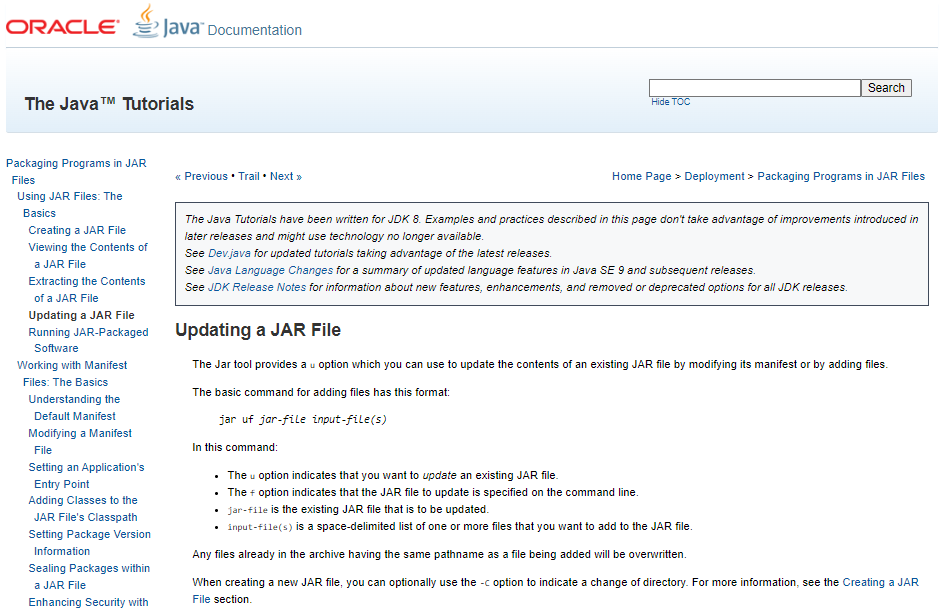
\includegraphics[width=\textwidth]{oracle-jar.PNG}
    \caption{Documentacion oficial de Oracle sobre como parchar un JAR}
    \label{hdfs.PNG}
\end{figure}

\noindent
A continuacion dejare el codigo original de WordCount y el codigo de ExtendedWordCount, hecho a partir del anterior.

\newpage

\begin{code}[H]
    \lstinputlisting[style=javastyle, caption={Codigo original de WordCount}, label={lst:002}]{code/WordCount.java}
\end{code}

\newpage

\begin{code}[H]
    \lstinputlisting[style=javastyle, caption={Codigo de ExtendedWordCount}, label={lst:002}]{code/ExtendedWordCount.java}
\end{code}

\newpage

\subsection{Implementación de selector de columna}

De la misma manera que el punto anterior, me base en WordCount para crear el codigo para la clase SelectColumnExtractor, el cual permite sustraer
una columna de la salida de WordCount en base al indice/numero de columna. Esta funcion en particular ejecuta WordCount si lo filtra al terminar
el proceso de Map-Reduce.

\newpage

\begin{code}[H]
    \lstinputlisting[style=javastyle, caption={Codigo de SelectColumnExtractor}, label={lst:002}]{code/SelectColumnExtractor.java}
\end{code}

\newpage

\subsection{Tiempo de ejecución}

\noindent
A continuación se muestran las medidas obtenidas utilizando el comando time en ExtendedWordCount:

\begin{table}[h!]
\centering
\begin{tabular}{lccc}
\toprule
\textbf{Archivo} & \textbf{real (s)} & \textbf{user (s)} & \textbf{sys (s)} \\
\midrule
sw-script-e04.txt  & 0m32.822s  & 0m7.653s & 0m0.388s
\bottomrule
\end{tabular}
\caption{Tiempos de ejecución del WordCount extendido}
\end{table}

\noindent
Luego se muestran las medidas obtenidas utilizando el comando time en SelectColumnExtractor:

\begin{table}[h!]
\centering
\begin{tabular}{lccc}
\toprule
\textbf{Archivo} & \textbf{real (s)} & \textbf{user (s)} & \textbf{sys (s)} \\
\midrule
sw-script-e04.txt  & 0m17.656s  & 0m7.137s & 0m0.350s
\bottomrule
\end{tabular}
\caption{Tiempos de ejecución del SelectColumnExtractor}
\end{table}

\noindent
Comparando ambos resultados, puedo concluir que:
\begin{itemize}
    \item El algoritmo de ExtendedWordCount es más intensivo en CPU, debido al preprocesamiento de texto, pero se mantiene eficiente gracias a la simplicidad del flujo MapReduce.
    \item El SelectColumnExtractor es más ligero y orientado a E/S, siendo más rápido en archivos simples, pero ligeramente mas costoso si las líneas contienen muchas columnas.
    \item Ambas soluciones escalan correctamente, pero el SelectColumnExtractor presenta tiempos de respuesta mas bajos en tareas estructuradas y simples.
\end{itemize}

\noindent
Los resultados se pueden ver en tiempo real en el video indicado al inicio del practico ({\color{blue}\href{https://github.com/apache/hadoop}{enlace}}).

\newpage

\section{Spark}

A continuacion se describe detalladamente el desarrollo de la tarea práctica avanzada de Big Data, basada en el uso de \texttt{Flintrock} para la configuración de un clúster Spark en AWS. 
A diferencia del informe original, este documento se enfoca en detallar todo el proceso personal, incluyendo errores cometidos, correcciones, decisiones de diseño, observaciones y comentarios 
adicionales que pueden ser útiles para otros estudiantes que enfrenten una tarea similar. Se proporciona ademas un video explicativo mostrando evidencia de el levantamiento de el informe y otros
detalles adicionales ({\color{blue}\href{https://www.youtube.com/watch?v=cp5aBbUCwiQ}{enlace}}).

Para comenzar, se utilizó el mismo clúster que se trabajó en la entrega inicial. Se eliminó manualmente todos los nodos worker, manteniendo solamente el nodo master. Este paso fue esencial para asegurar una base limpia antes de implementar una nueva configuración.

Se clonaron los siguientes repositorios proporcionados por el profesor:
\begin{itemize}
    \item \texttt{https://github.com/ptoledo-teaching/training-bigdata-002}
    \item \texttt{https://github.com/nchammas/flintrock}
\end{itemize}

Estos repositorios contienen scripts clave para la creación del clúster. Se realizó una navegación rápida con \texttt{tree} y \texttt{vim} para entender su estructura y funcionalidades.

El proceso de instalación incluyó los siguientes pasos:
\begin{enumerate}
    \item Instalación de \texttt{AWS CLI}.
    \item Instalación de \texttt{pipx}.
    \item Instalación de \texttt{Flintrock} mediante \texttt{pipx}.
\end{enumerate}

Durante este proceso, se descubrió que el script contenía una instrucción para crear un rol IAM para S3, pero el profesor indicó que esto no era necesario. Por ende, se omitió este paso aunque inicialmente se intentó (sin éxito, debido a permisos insuficientes).


Se detectó un bug en la versión actual de Flintrock relacionado con incompatibilidades de Spark. Para solucionarlo, se aplicó un parche manualmente en el código fuente de Flintrock instalado. El procedimiento incluyó:
\begin{itemize}
    \item Edición directa de los archivos indicados por el profesor.
    \item Verificación y corrección de problemas de indentación (uso de tabs vs. espacios).
    \item Uso de expresiones regulares para reemplazo masivo.
\end{itemize}

\textbf{Nota:} Se olvidó hacer un respaldo del archivo original antes de modificar, lo que pudo haber provocado una reinstalación completa en caso de error.

Se creó una nueva clave PEM con permisos adecuados y se renombró según el formato requerido por Flintrock. Inicialmente se cometió un error en los permisos, generando un \texttt{warning}. Posteriormente se corrigió con:

\begin{lstlisting}[language=bash]
chmod 400 clave.pem
\end{lstlisting}

Esto permitió una conexión exitosa al nodo master.

\subsection{Escalamiento vertical y horizontal}

Se procedió a levantar múltiples configuraciones de clúster usando archivos \texttt{.yaml} modificados. Se observó que configuraciones con más de 8 nodos fallaban debido a restricciones de la cuenta de estudiante. Por lo tanto, se trabajó principalmente con configuraciones de hasta 6 nodos \texttt{t3.large}.

\begin{itemize}
    \item Configuración con 10 \texttt{t3.medium} no logró levantar el clúster.
    \item Ejecute el script \texttt{test-000.sh} en lugar de \texttt{test-001.sh}, generando inconsistencias en los benchmarks.
\end{itemize}

\subsection*{Tiempos Registrados}

\begin{longtable}{|c|c|c|}
\hline
\textbf{Configuración} & \textbf{Test Ejecutado} & \textbf{Tiempo Aproximado} \\
\hline
4 \texttt{t3.large} & test-000.sh & 24 (real) \\
\hline
4 \texttt{t3.large} & test-000.sh & 24 (real) \\
\hline
4 \texttt{t3.small} & test-000.sh & 25 (real) \\
\hline
6 \texttt{t3.micro} & test-000.sh & 25 (real) \\
\hline
6 \texttt{t3.small} & test-000.sh & 26 (real) \\
\hline
10 \texttt{t3.medium} & test-000.sh & Falló (fallaba en launch.sh) \\
\hline
\end{longtable}

\textit{Nota:} Los tiempos fueron medidos usando el comando \texttt{time bash test00.sh}, y registrados manualmente en un bloc de notas para su análisis posterior.

\section{Procesamiento de datos}

\subsection{Extracción, transformación y carga}

{\color{red} Desarrolle un programa basado en el test-001 que permita la extracción, transformación y carga (extraction, transformation and load, normalmente denominado ETL) del dataset de la asignatura. El set total de datos de la asignatura corresponde al archivo de 7.2[GB] disponible en \url{s3://utfsm-inf356-datasets/vlt_observations/vlt_observations.csv}. Este dataset ha sido dividido en 20 segmentos con nombre \url{s3://utfsm-inf356-datasets/vlt\_observations/vlt_observations_XXX.csv} para poder disponer de un acceso fraccionado a los datos.

    El proceso ETL debe procesar el dataset entregado y generar un nuevo dataset para procesamiento posterior, el que debe considerar las siguientes columnas:
    \begin{itemize}
        \item Right ascension - grados
        \item Right ascension - minutos
        \item Right ascension - segundos
        \item Declination - grados
        \item Declination - minutos
        \item Declination - segundos
        \item Instrument
        \item Exposition time
        \item Template start (en tiempo unix)
    \end{itemize}

    El dataset procesado sólo debe tener los registros que corresponden a las observaciones con categoría  SCIENCE y tipo de observación OBJECT (referencia \url{https://archive.eso.org/eso/eso_archive_help.html}).

    El resultado del dataset debe ser guardado en formato parquet en la raíz de su bucket de desarrollo bajo el nombre \textbf{vlt\_observations\_etl.parquet}. Se solicitará incluir el código bajo el nombre code-005.py en su entrega. Describa el procedimiento y muestre alguna métrica relativa a la ejecución y/o resultado de su procedimiento.}

\begin{code}[H]
    \lstinputlisting[style=pythonstyle, caption={Código utilizado para el procedimiento de ETL}, label={lst:005}]{code/code-005.py}
\end{code}

\subsection{Coordenadas galácticas}

{\color{red} Desarrolle un programa que lea el archivo generado por el proceso ETL y genere un nuevo archivo parquet en el que se han transformado las coordenadas RA-DEC ecuatoriales de las observaciones a coordenadas galácticas. El nuevo archivo debe estar en la raíz de su bucket de desarrollo y debe ser llamado \textbf{vlt\_observations\_gc.parquet}. El archivo debe tener las columnas:
    \begin{itemize}
        \item Galactic right ascension (float en grados)
        \item Galactic declination (float en grados)
        \item Instrument
        \item Exposition time
        \item Template start (en tiempo unix)
    \end{itemize}
    Se solicitará incluir el código bajo el nombre code-006.py en su entrega. Describa el procedimiento y muestre alguna métrica relativa a la ejecución y/o resultado de su procedimiento.}

\begin{code}[H]
    \lstinputlisting[style=pythonstyle, caption={Código utilizado para el cálculo de coordenadas galácticas}, label={lst:006}]{code/code-006.py}
\end{code}

\subsection{Segmentación temporal}

{\color{red} Segmente el archivo de coordenadas galácticas en tantos archivos como sea necesario de modo de contar con una agrupación por año y por semana del año. Se considera la primera semana del año la semana del primer lunes de un año. Los primeros días del año pertenecen al año anterior si ocurren antes del primer lunes del año.

    Los datos deben ser guardados en formato parquet en una carpeta llamada \textbf{partition} en la raiz de su bucket de desarrollo. Dentro de partition las carpetas se separarán por año. Dentro de la carpeta de un determinado año deberá haber un archivo denominado \textbf{vlt\_observations\_XXXX.parquet} con todos los datos del año, y una carpeta denominada weeks, que dentro debe tener una serie de archivos denominados \textbf{vlt\_observations\_XXXX\_YY.parquet}, donde XXXX corresponde al año y YY al número de semana comenzando en 0.

    Se solicitará incluir el código bajo el nombre code-007.py en su entrega. Describa el procedimiento y muestre alguna métrica relativa a la ejecución y/o resultado de su procedimiento.}

\begin{code}[H]
    \lstinputlisting[style=pythonstyle, caption={Código utilizado para segmentación temporal de datos}, label={lst:007}]{code/code-007.py}
\end{code}

\subsection{Conteo de observaciones}

{\color{red} Desarrolle un programa que reciba un archivo parquet con el formato previamente utilizado para las coordenadas galácticas y que genere un conteo de las observaciones para cada segmento de 10 grados horizontal y vertical del cielo, segmentado por cada instrumento. El archivo de salida debe tener el mismo nombre que el archivo de entrada pero con un .count antes de la extensión .parquet. El conteo tiene que tener como coordenada de referencia el centro de la región angular. El tiempo de exposición debe ser reemplazado por el tiempo total de observaciones que han sido considerados en la cuenta. Se debe descartar la columna con el tiempo de inicio del template.

    Se solicitará incluir el código bajo el nombre code-008.py en su entrega. Describa el procedimiento y muestre alguna métrica relativa a la ejecución y/o resultado de su procedimiento.}

\begin{code}[H]
    \lstinputlisting[style=pythonstyle, caption={Código utilizado para segmentación temporal de datos}, label={lst:007}]{code/code-008.py}
\end{code}

\end{document}
